
\documentclass[11pt,final,twocolumn]{IEEEtran}
\usepackage{graphicx}
\usepackage{expdlist}
\usepackage{fancyvrb}
\usepackage{float}

\renewcommand{\figurename}{Figure}
\renewcommand{\thefigure}{\Roman{figure}}
\restylefloat{pc}
\floatname{pc}{Figure}
\newfloat{pc}{H}{lop}
\setlength{\parindent}{0pt}
\setlength{\parskip}{1ex}
\begin{document}

\title{Image Processing Technique for Automated Viral Plaque Counting}
\author{Michael Moorman, Aijuan Dong \\
Hood College}
\maketitle
\section{Abstract}
The viral plaque assay is an important procedure in virology. One step of this procedure includes the manual counting of viral plaques with the naked eye.  This is often a time consuming and laborious process. A method is presented for automating viral plaque counting using image processing techniques and the OpenCV Computer Vision library. The method consumes an image of an entire plate of viral plaque samples and outputs individual counts of each sample in the plate. The image is captured using a commercial flat bed scanner. Experimental results show that the method is up to 90 percent accurate in comparison to trained human counts. The program produces results for a single image in about one second.  Compared to commercial colony counter systems, the proposed method is extremely economical; the only hardware required by the method is a personal computer and a flatbed scanner.  Finally, an open source implementation of the program is provided, which includes an optional graphical user interface. 



\section{Introduction}
The viral plaque assay is an important and commonly used procedure in biology; however, a stage of the process requires that a person manually count the instances of plaque structures . The work presented here attempts to accurately count mammalian  viral plaques using image processing techniques. The image below is a typical example of an input image.
\begin{figure}[h]
\centering
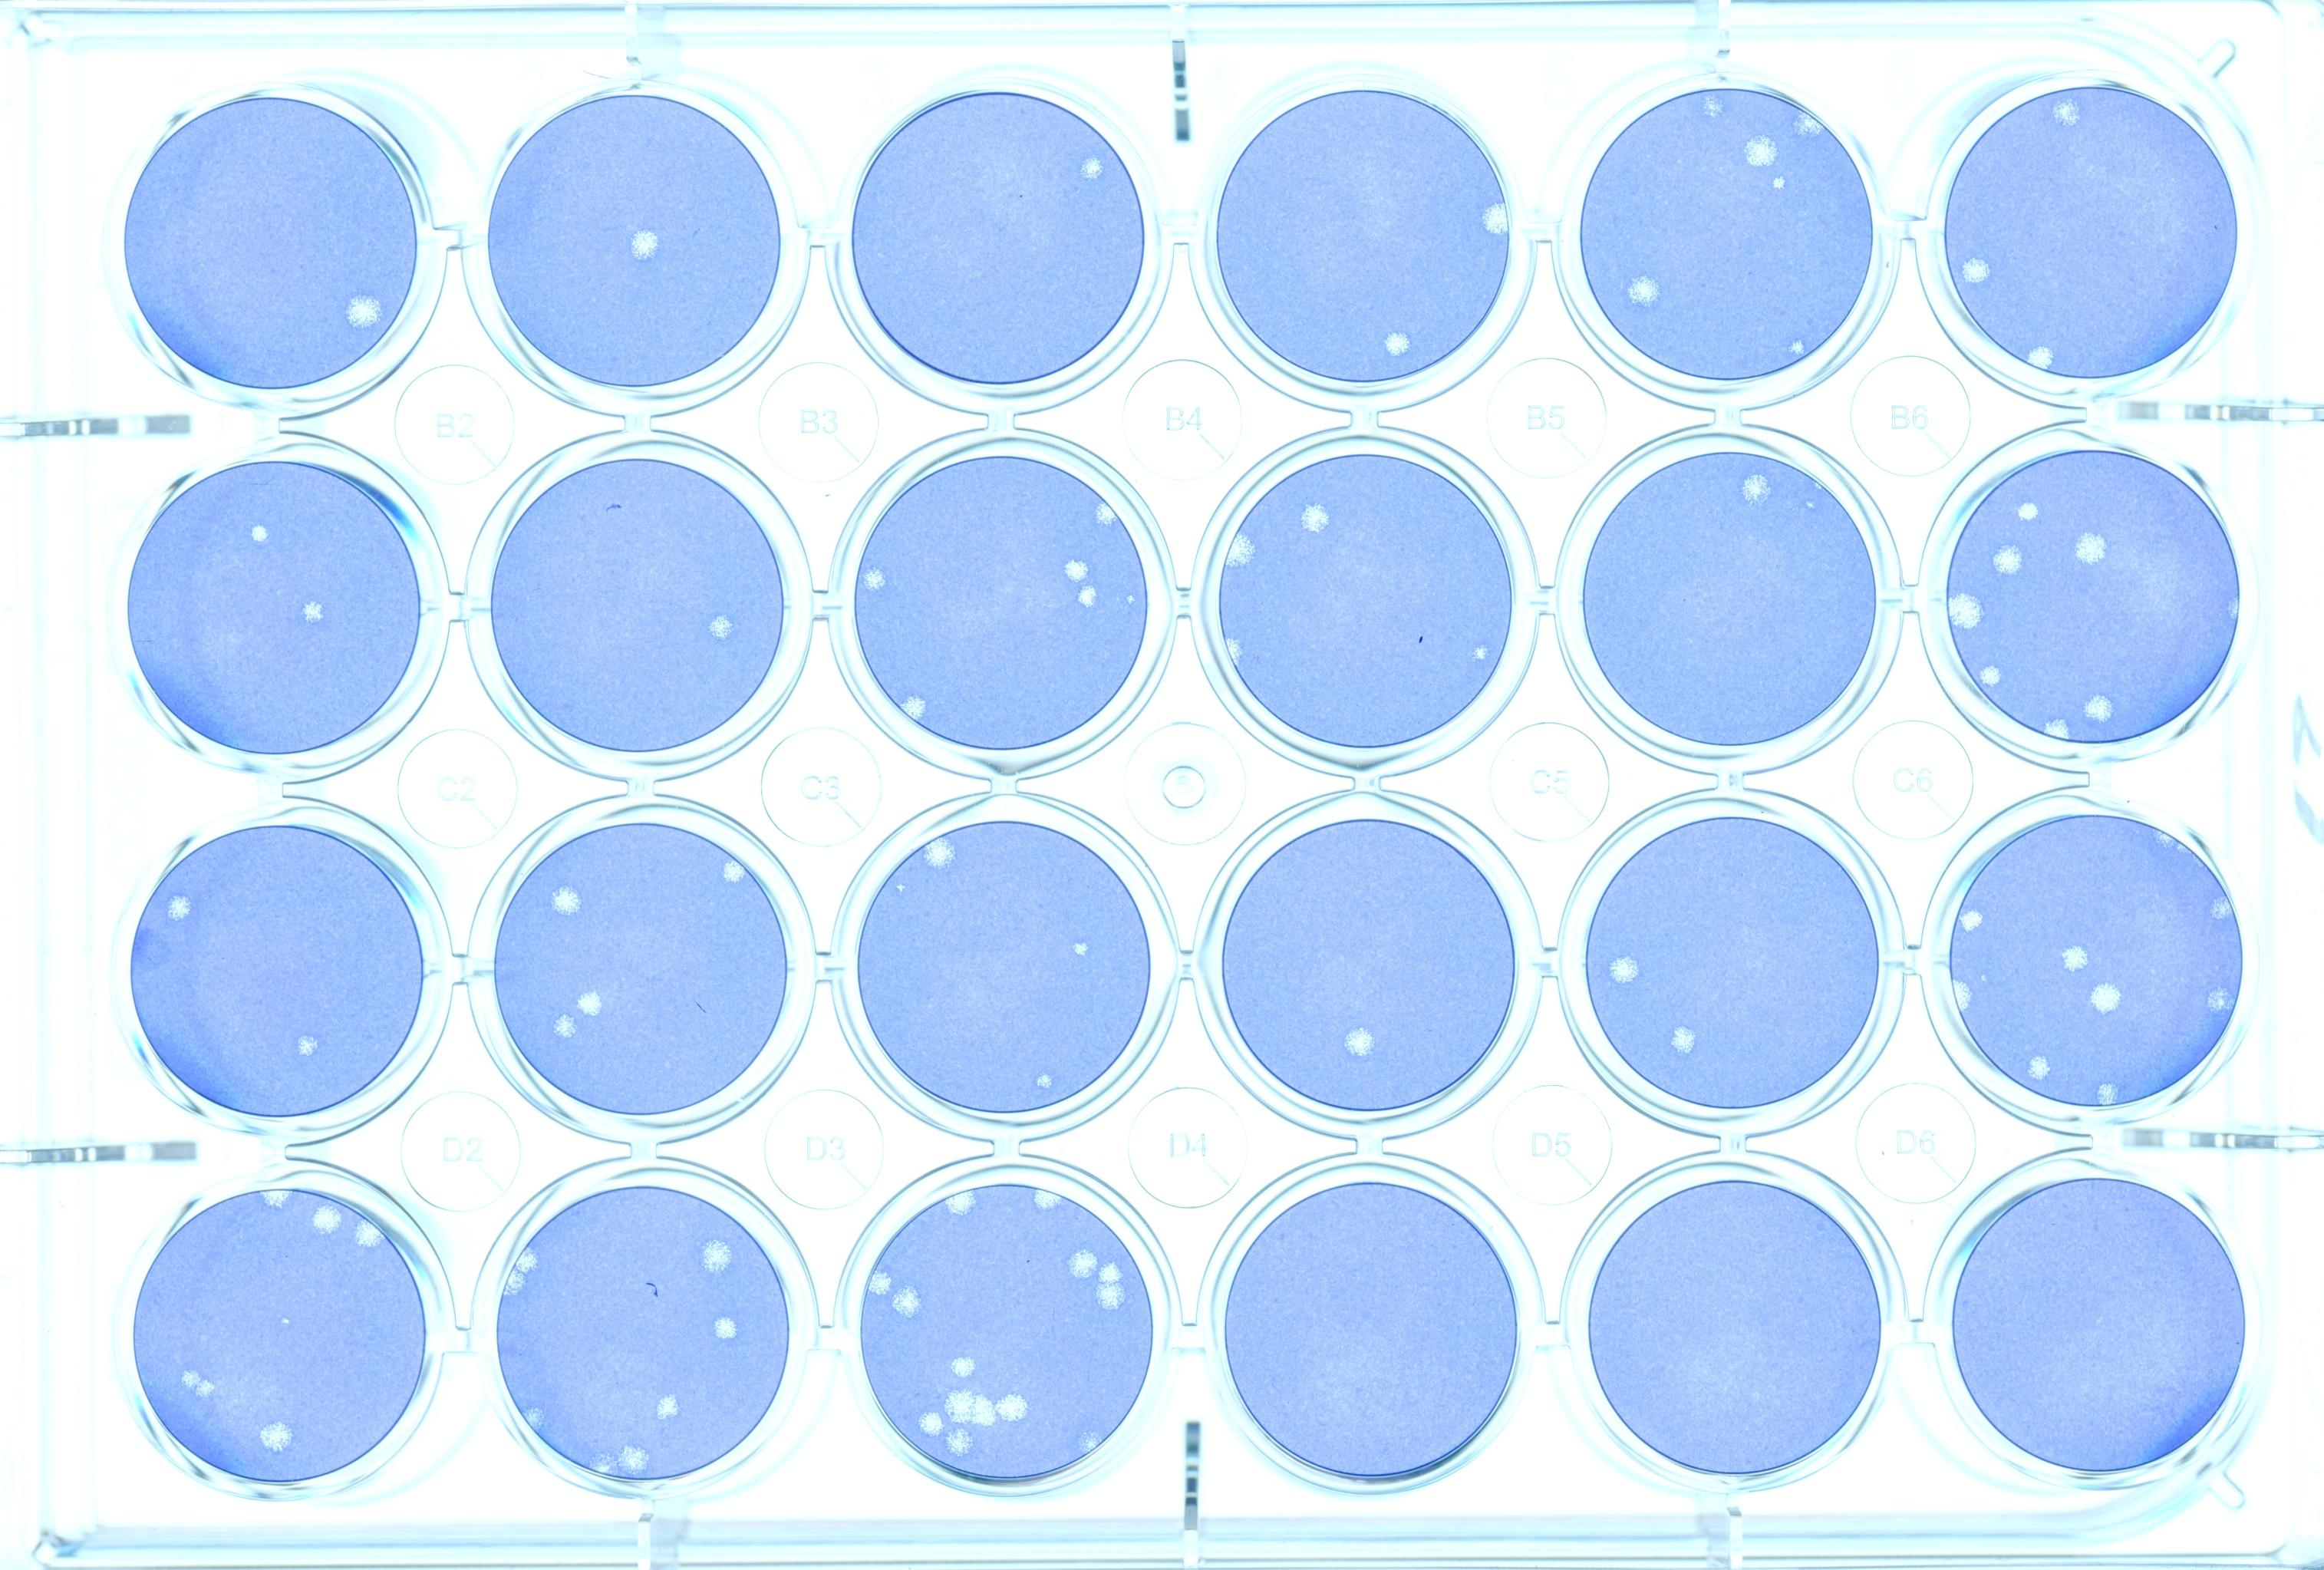
\includegraphics[width=.4\textwidth]{sample.jpg}
\caption{A typical example of a viral plaque image}
\label{fig:sample}
\end{figure}


A common example of the procedure begins by preparing several dilutions of a virus stock. Tissue plates, arranged in a batch of 6x4 wells, are configured with a thin monolayer of susceptible animal tissue sample.  The wells are then innoculated using the various virus dilutions. After inncoulation, the wells are topped off with a special agar that limits viral expansion to only neighboring cells. Each sample is allowed to incubate for some amount of time, allowing the virus to attack the cells In the monolayer. Over time, the virus gradually destroys neighboring cells, creating visible structures also known as viral plaques. The visibility of these plaques are sometimes enhanced with the usage of special dyes. Once the plaques have grown large enough to be seen by the naked eye, the titer of the original virus stock is discovered by observing the number of  plaque-forming units (PFU) per milliliter present in each well.

The last stage of this procedure can be particularly laborious . Counts  of the number of plaque formations on each well are manually tallied by hand. In a typical case, a sample can contain over 100 viral plaques. It is easy to see how tallying an entire plate of samples often consumes several minutes of someones time. 


Automated counting of viral plaques via image processing techniques  has been proposed and investigated many times before, and there are several commercial products on the market that manufacture colony counting systems. [CITE].  There is a lucrative market for automated colony counting, and several companies manufacture colony counting systems. Some of these systems can cost thousands of dollars and are often both closed source and not economically feasible. [CITE] . Other studies have approached automated viral plaque counting before and have tried a number of different  approaches. Some of these include use of a Watershed Transform [CITE], Distance transform[CITE],  Hough transform[CITE], parameter identification and fuzzy logic. Of these works, However,  they did not feature the ability to process an entire plate of samples. 

At present time,  there is not a low cost and  accurate colony counting system available that enjoys wide spread adoption and that is able to accommodate an entire plate of samples. This is a primary motivation for the work presented here. In addition, the performance of some of these works was poor. In the case of [CITE], the system consumed ten seconds of wall clock computational time to analyze a single viral plaque plate. 

Accurately counting plaques in these types of images presents several challenges. Perhaps the most difficult challenge that any solution must address is how to deal with the noise in the image.  How does one go about discerning the difference between viral plaques and the frequent noisy particles in the agar of the plates?  This is particularly problematic when dealing with small plaques, as there signal to noise ratio is very small in that case.  

OpenCV is an open source computer vision library available from http://sourceforge.net/projects/opencvlibrary. The library is written in C and C++ and runs under Linux, Windows, and Mac OS X. It provides an application interface (API) that this study uses to implement the proposed method. 


\section{Methodology}
The proposed method is implemented as a computer program written in C++ and uses the  OpenCV [CITE] image processing API to perform image analysis. 

\subsection{User Supplied Parameters}
The user supplies the program with an image of a plate of viral plaques, and also specifies three parameters.
\subsubsection{Well radius}
The radius of each well, given in pixels.

\subsubsection{Minimum Plaque Radius}
 The minimum radius of a viral plaque structure, given in pixels.

\subsubsection{Maximum Plaque Radius}
 The maximum radius of a viral plaque structure, given in pixels.


The method uses these parameters and a series of procedural morphological image transformations to ultimately produce viral plaque counts.

\subsection{Image Aquisition}
Image acquisition  is the first stage of the method. A flat bed scanner is used to capture an image of a plate of viral plaque samples, and they are encoded into an image file. 

\subsection{Segmentation}
Segmentation in the next stage of the method. The only interesting parts of the image lay within each well. Segmentation is an essential step that attempts to create a mask that shadows every part of the image that is not with in the barriers of a well on the plate. 

Perhaps the most difficult problem that segmentation seeks to resolve is the plate orientation problem. Image acquisition makes no guarantees as to the position of the plate with relation to the scanner surface. Plates may be butted up against the top left corner of the scanner, have a slight offset on any axis, or have any slight orientation about them, etc. A global segmentation approach overcomes these challenges. This approach is summarized below.

\begin{enumerate}
\item Grayscale the image.
\item Use Otsu's thresholding method [CITE] to transform the image into a binary image. This is depicted in figure \ref{fig:segOtsu}.
\begin{figure}[H]
\centering
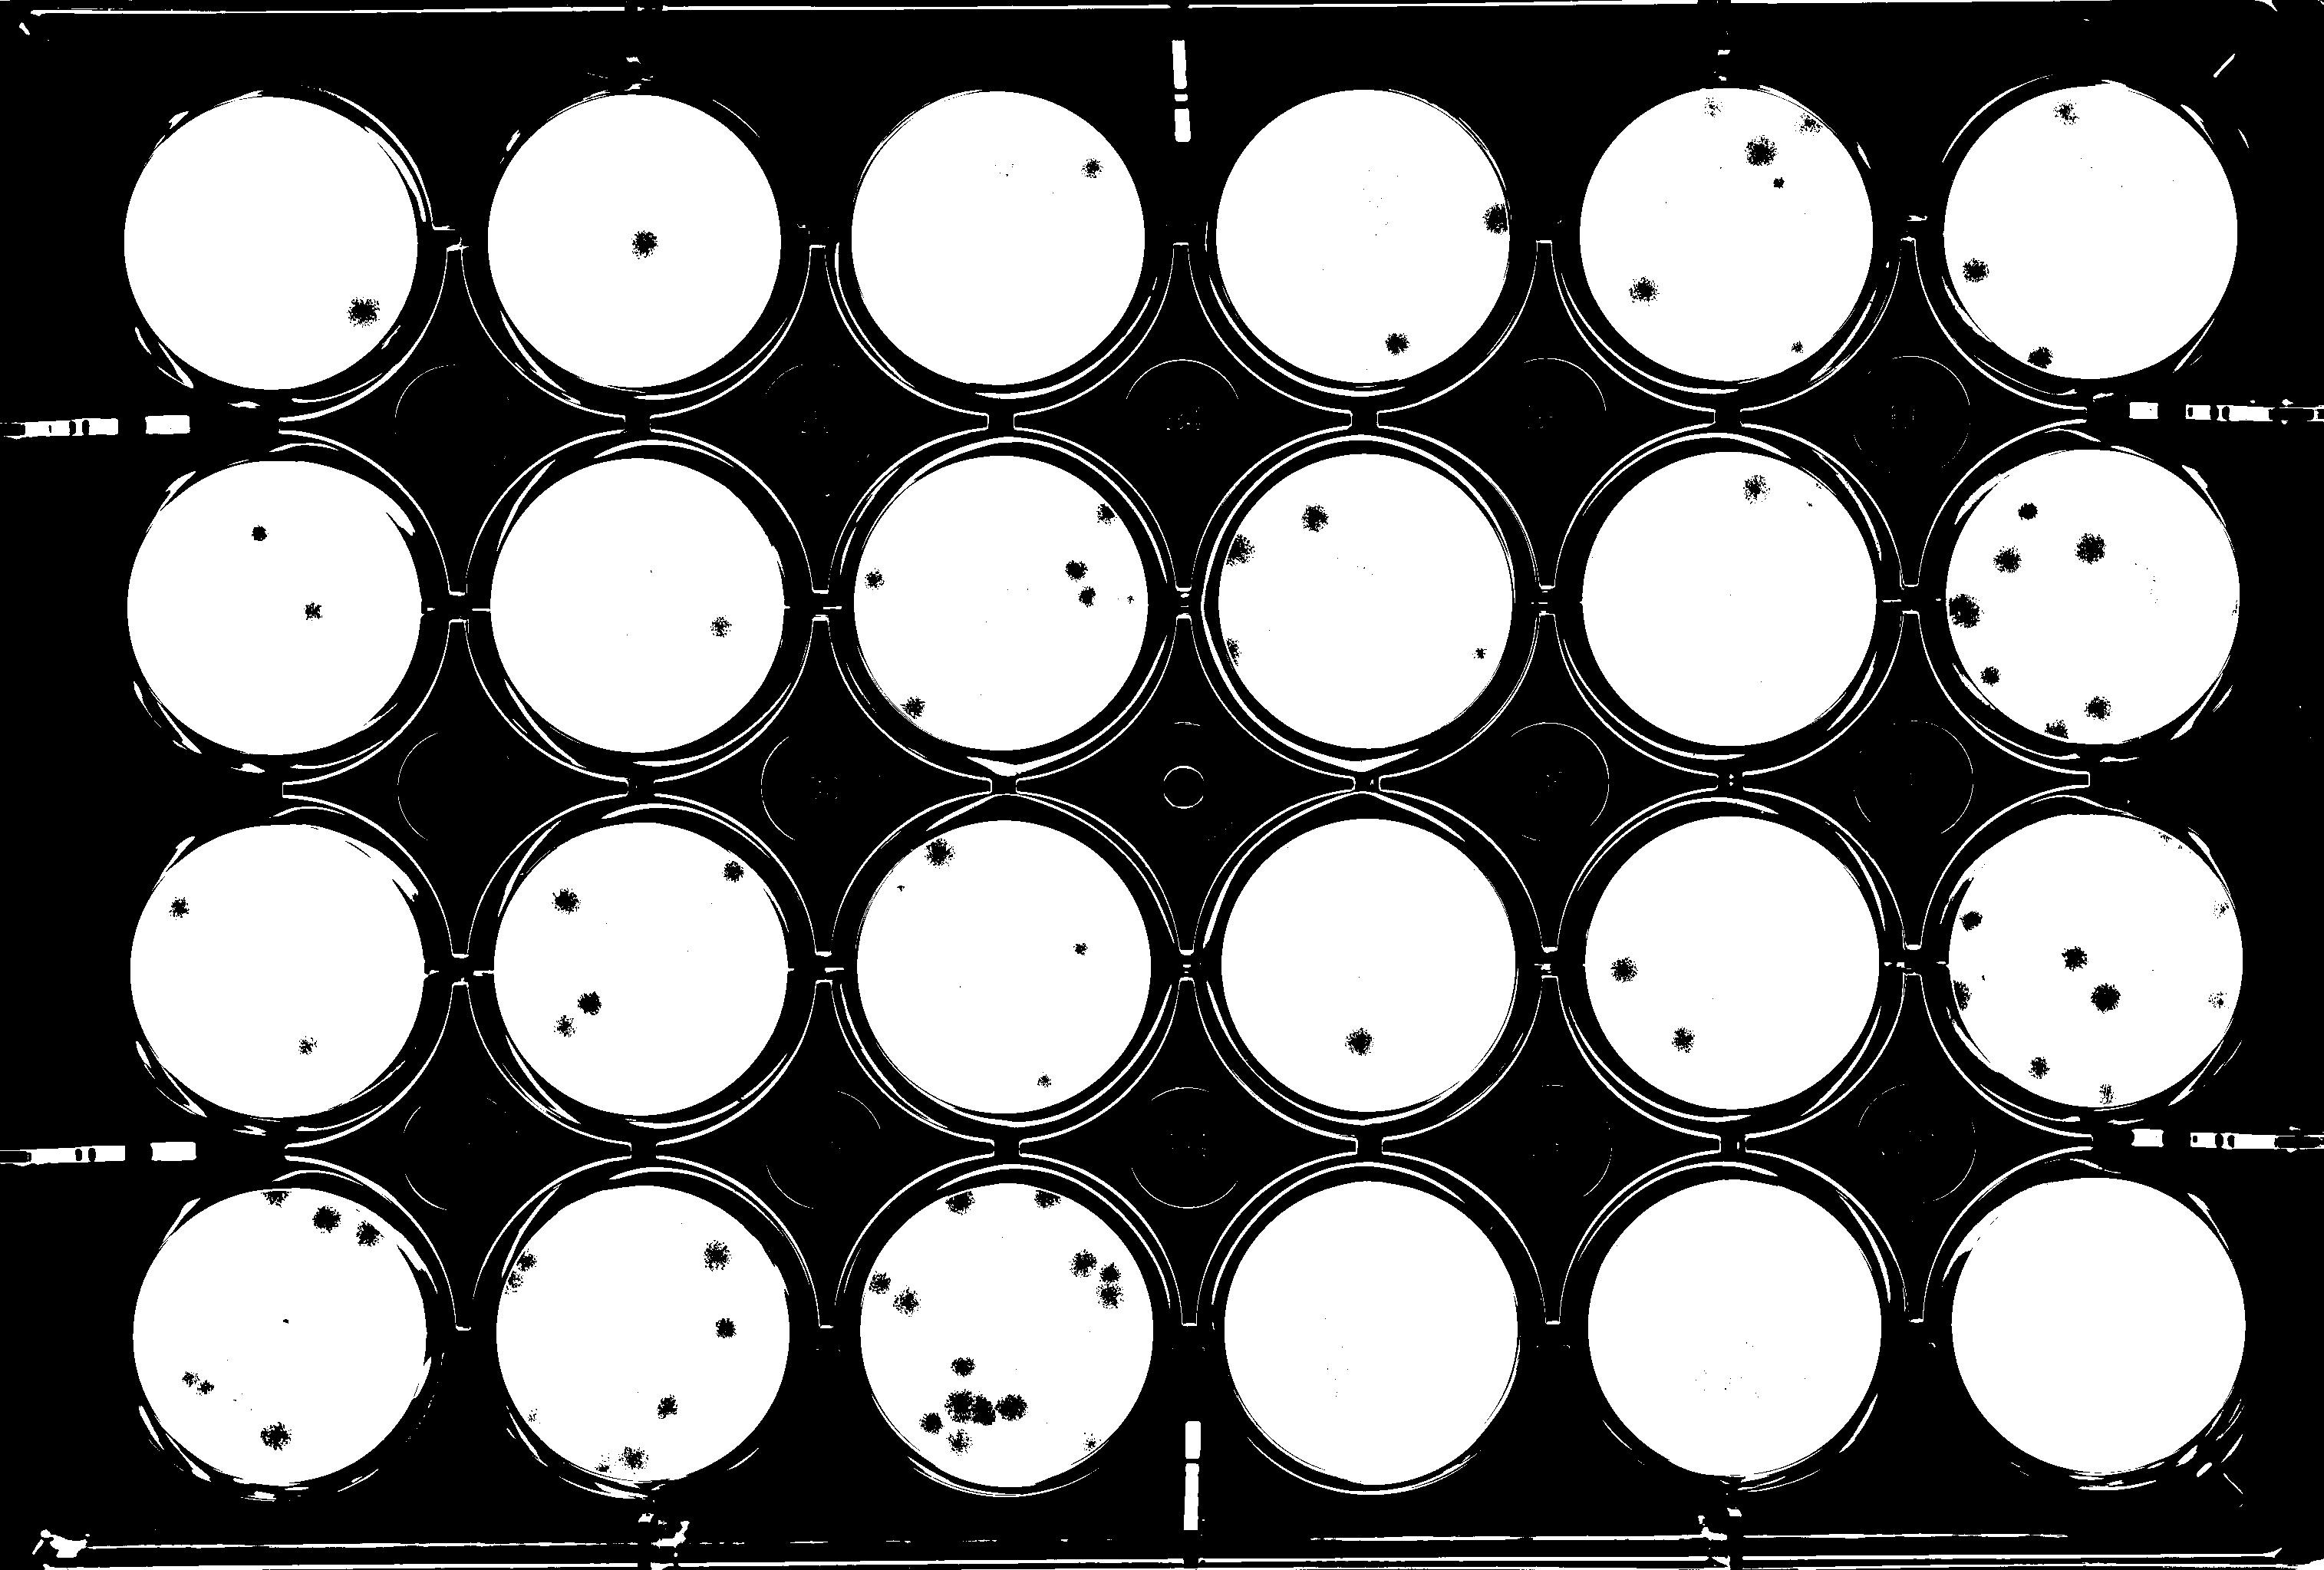
\includegraphics[width=.4\textwidth]{segmentOtsu.jpg}
\caption{Otsu thresholding}
\label{fig:segOtsu}
\end{figure}


\item
Perform a morphological dilation on the image that is sufficient enough to close viral plaque holes. This is shown in figure \ref{fig:segFillHoles}.
\begin{figure}[H]
\centering
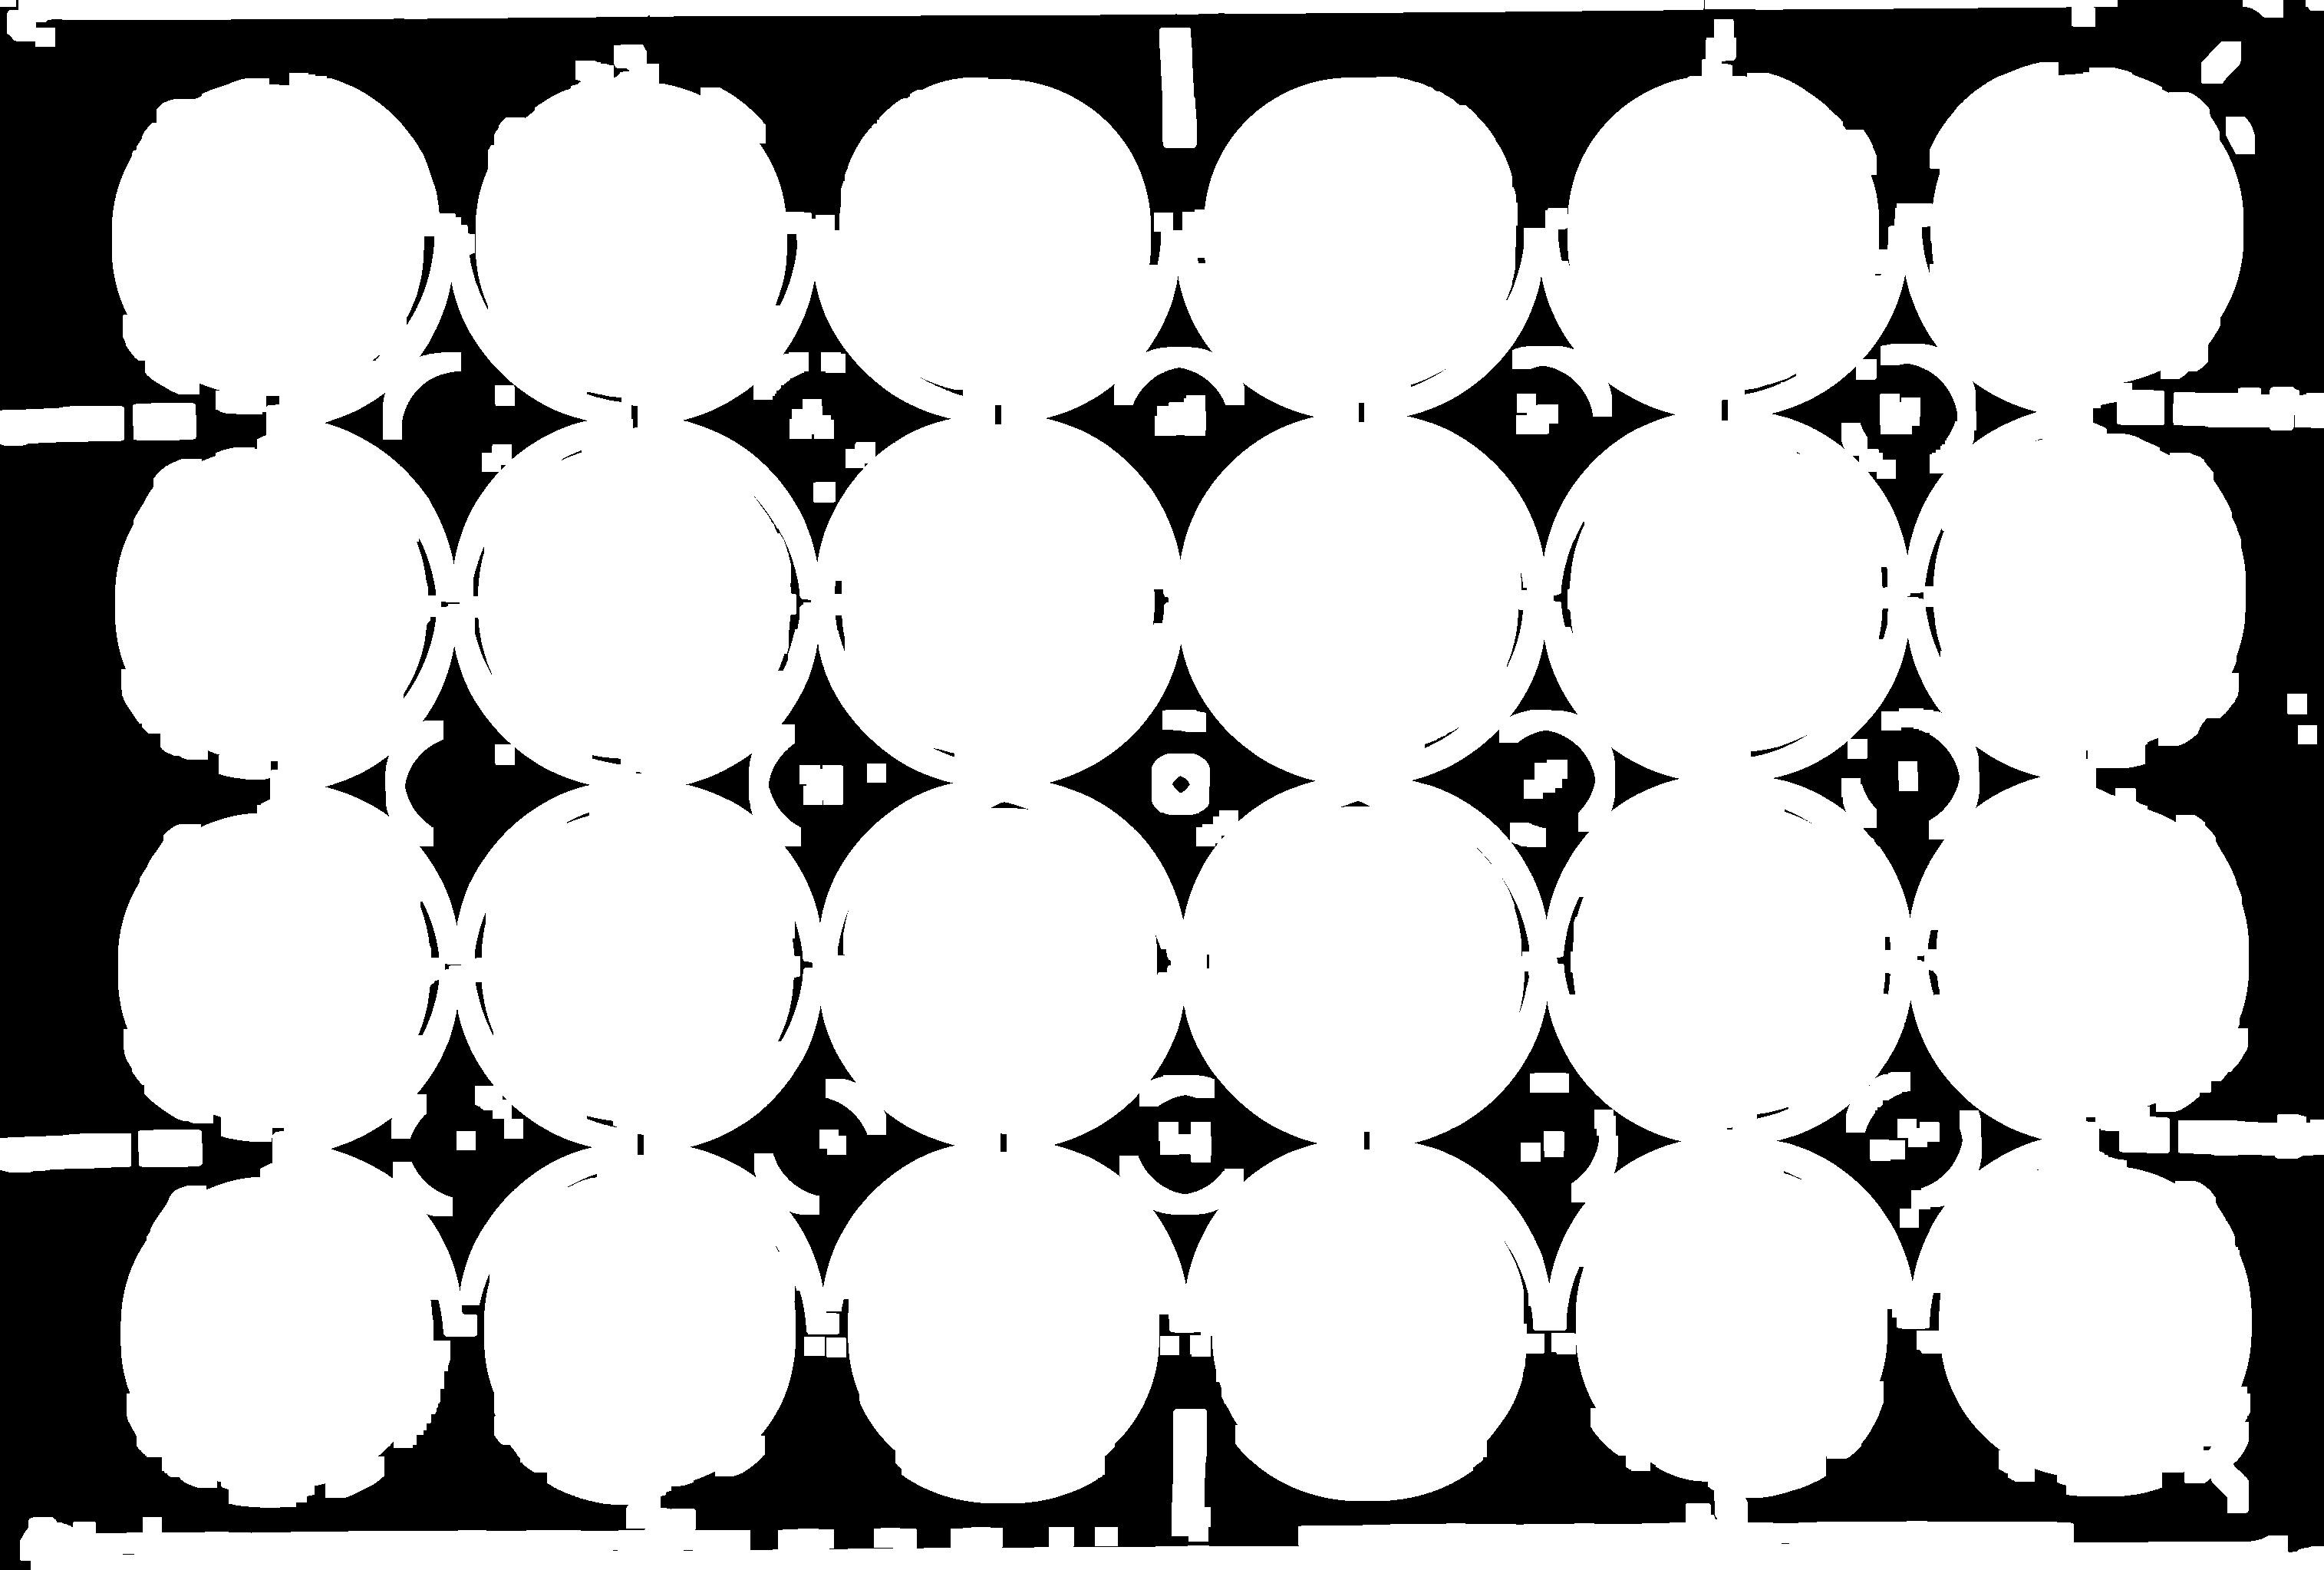
\includegraphics[width=.4\textwidth]{segmentFillHoles.jpg}
\caption{Use of dilation to fill holes.}
\label{fig:segFillHoles}
\end{figure}



\item
Aggressively perform several iterations of morphological erosion on the image until the number of artifacts that remain on the image equal the number of wells on the plate. This is shown in figure \ref{fig:segErode}.
\begin{figure}[H]
\centering
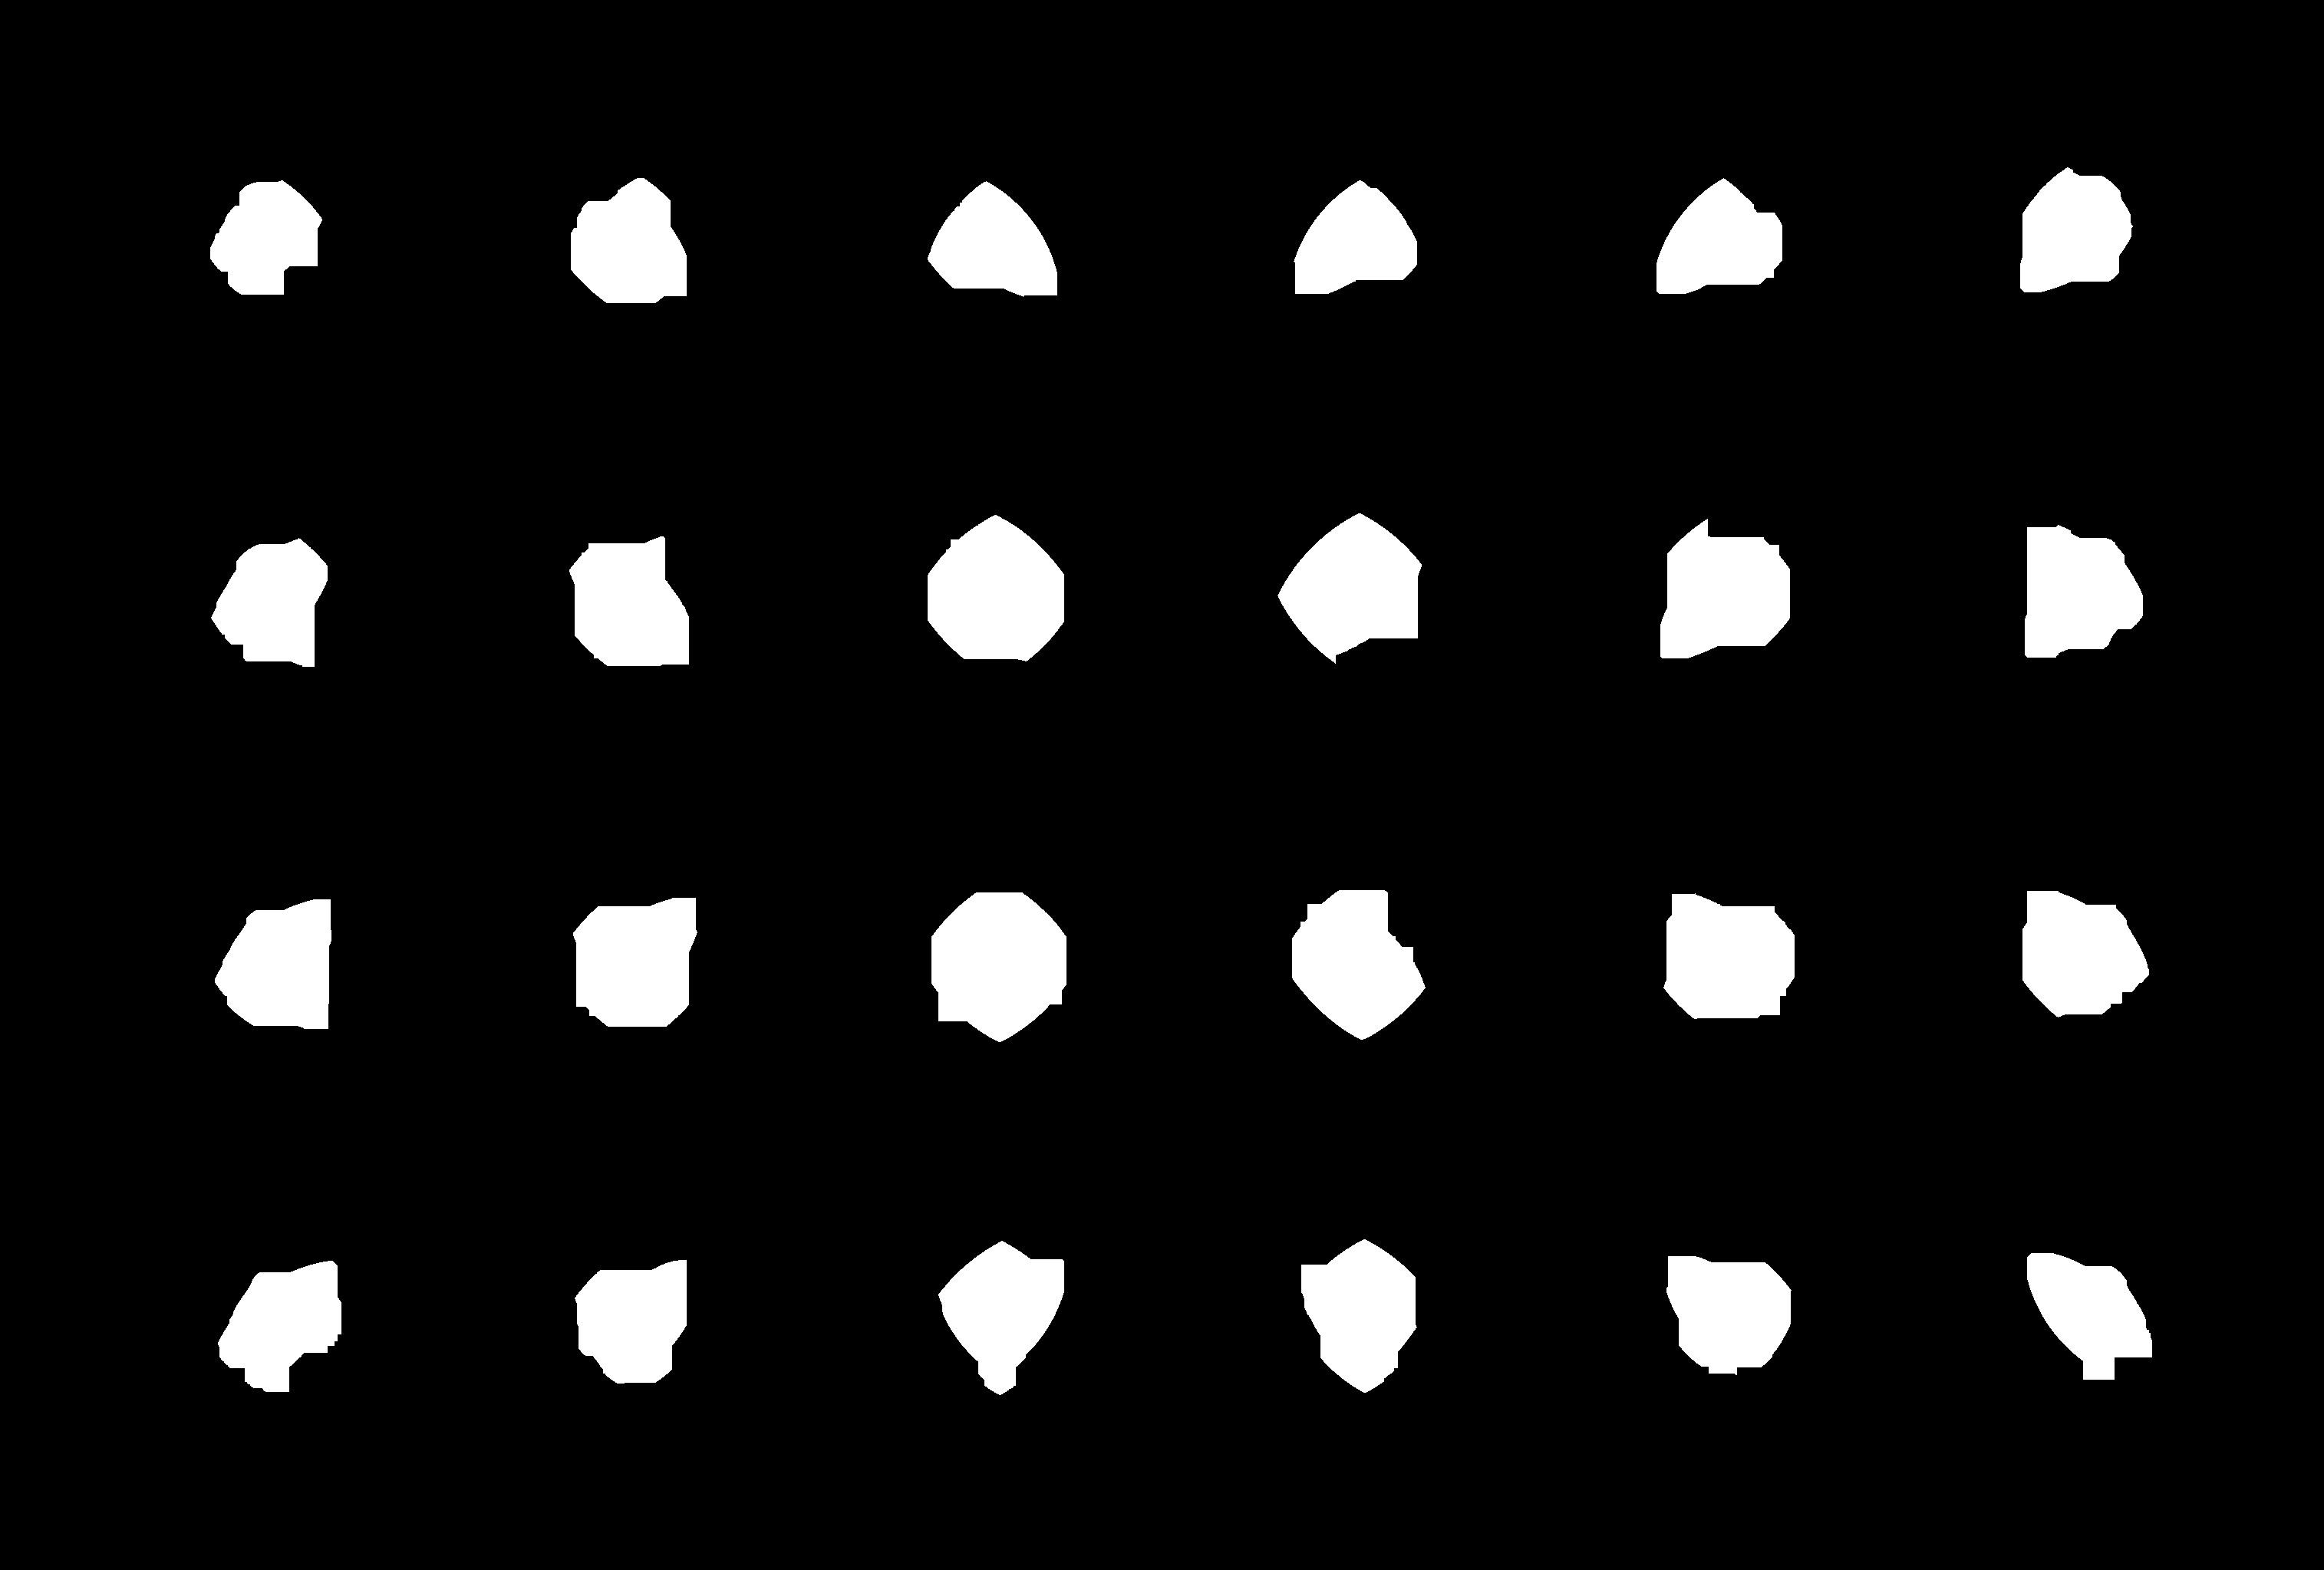
\includegraphics[width=.4\textwidth]{segmentErode.jpg}
\caption{Use of massive erosion}
\label{fig:segErode}
\end{figure}


\item
Calculate the center points of each remaining artifact. Use these points as seeds for a flood fill [CITE] operation that grows the region outward from each of these points on an RGB thresholded rendering of the original image.
Aggressively perform several iterations of morphological erosion on the image until the number of artifacts that remain on the image equal the number of wells on the plate. This is shown in figure \ref{fig:segFloodFill}.
\begin{figure}[H]
\centering
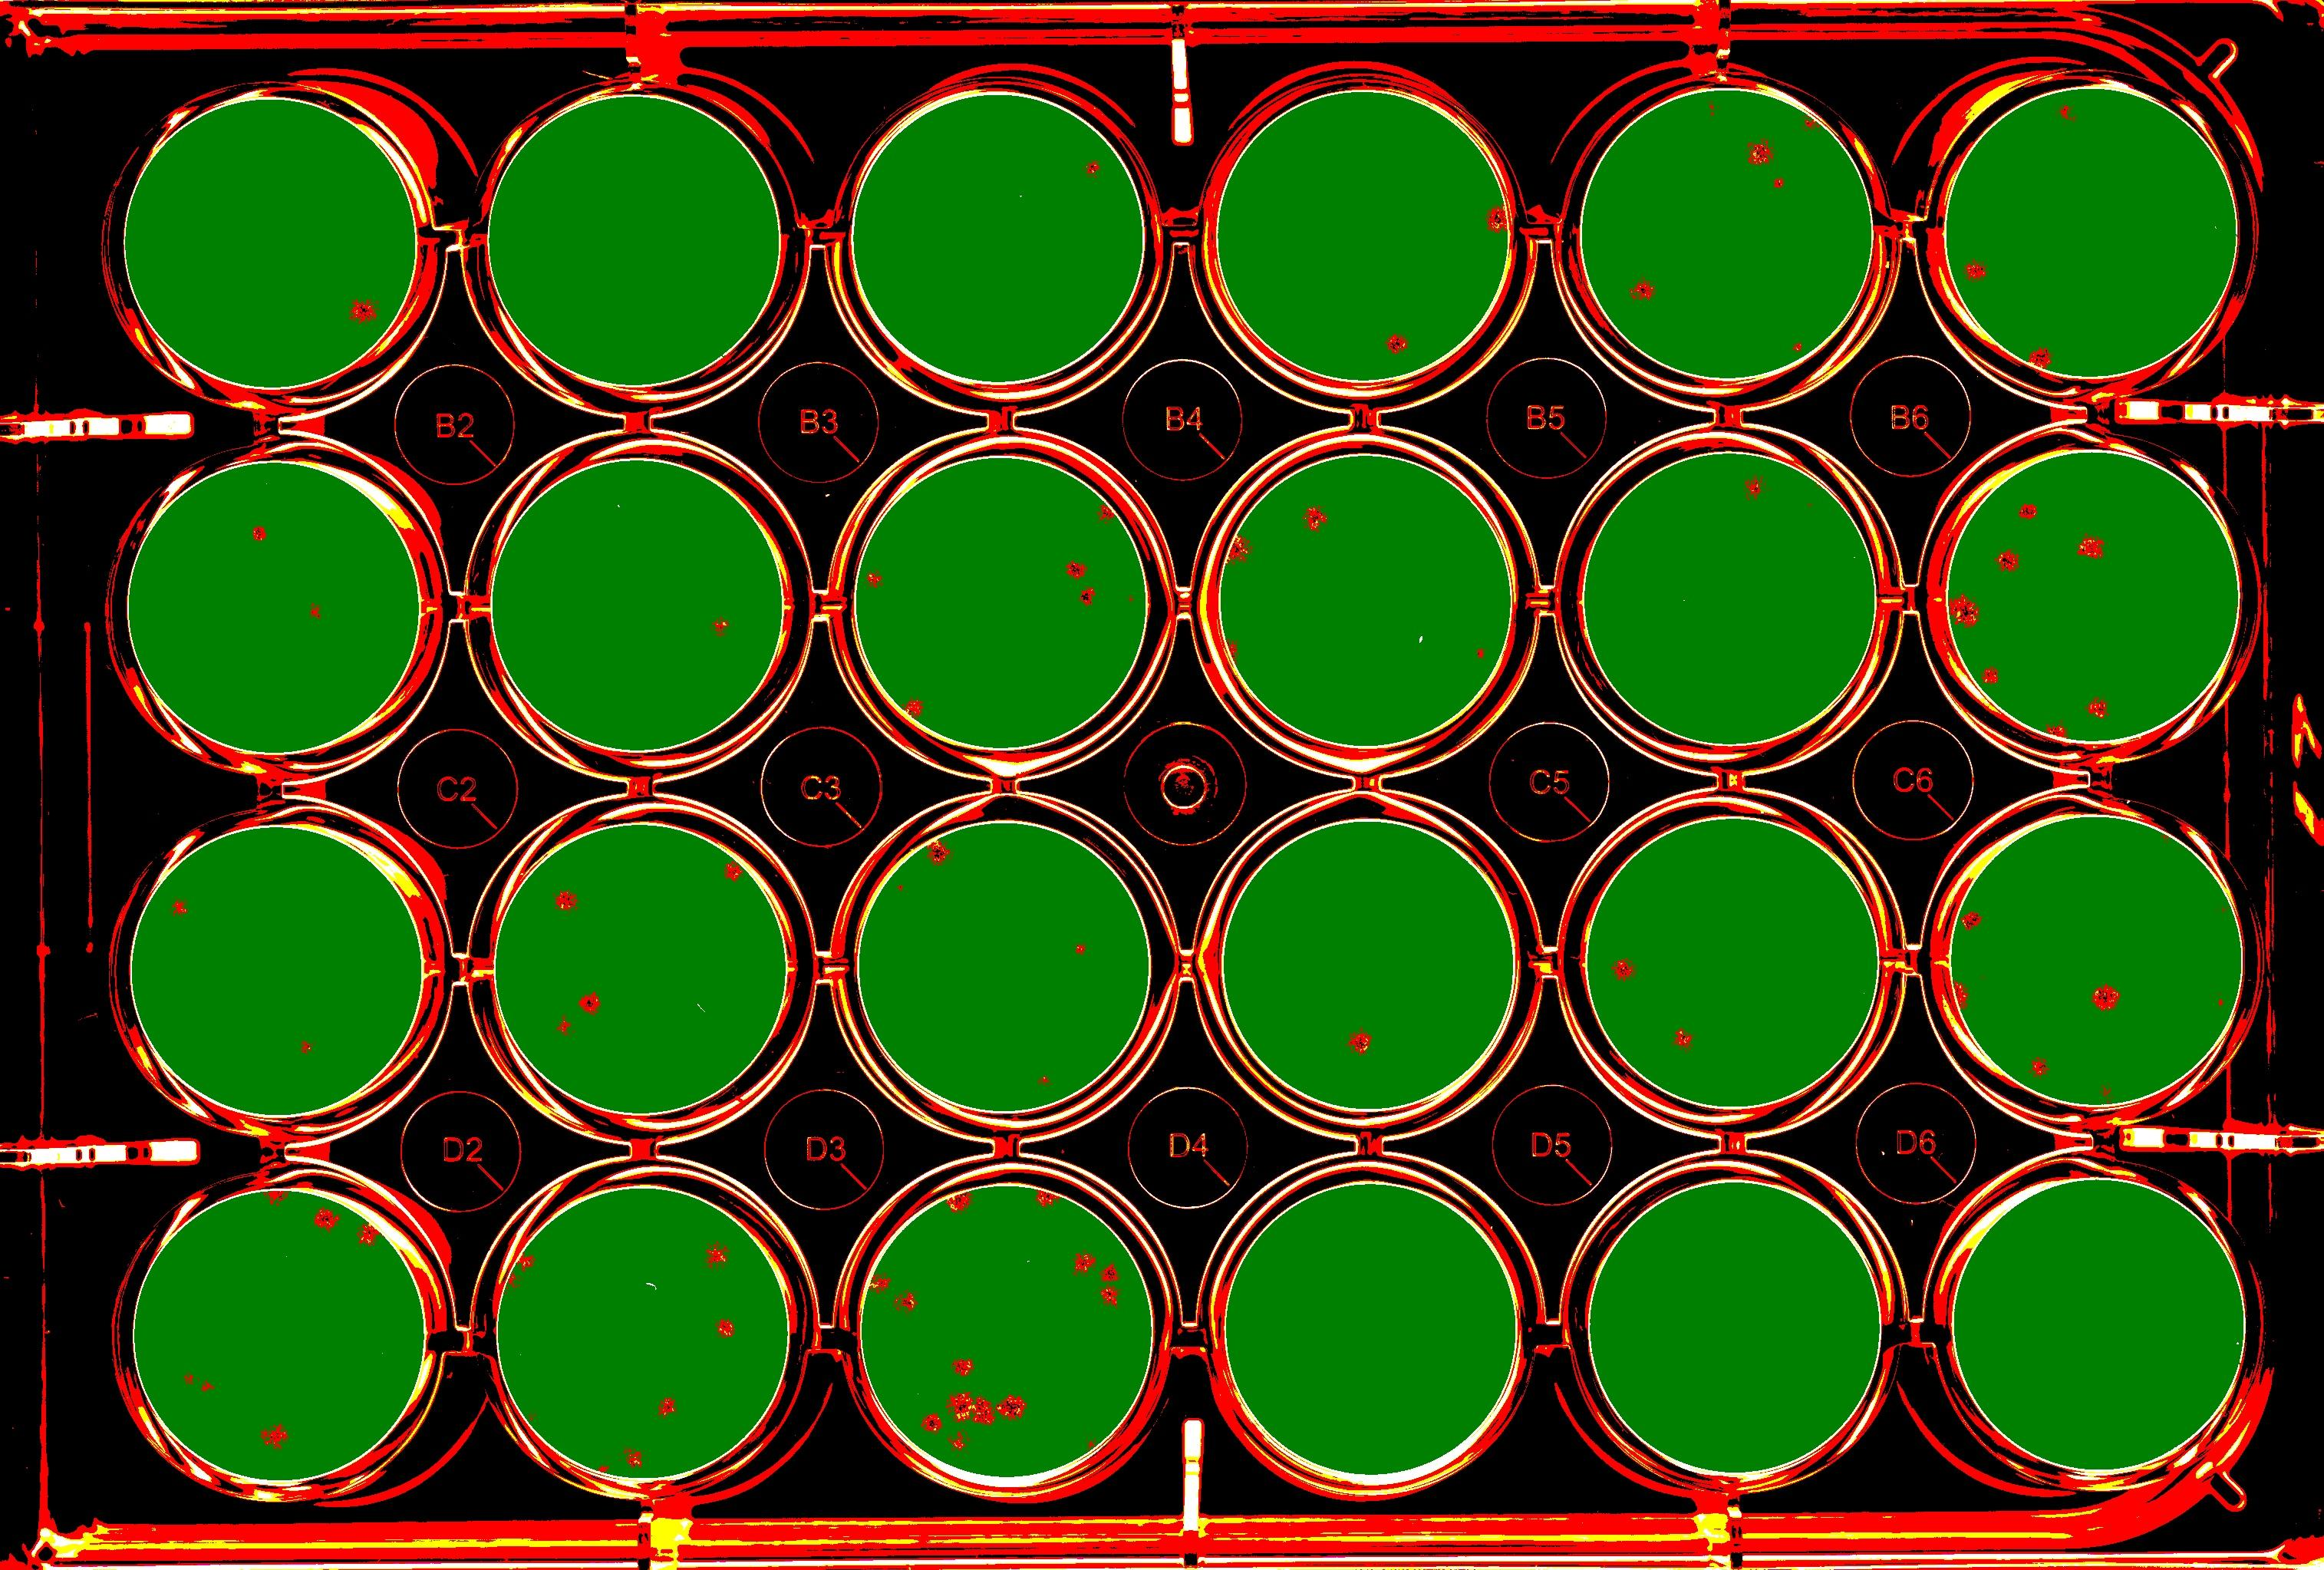
\includegraphics[width=.4\textwidth]{segmentFloodFill.jpg}
\caption{Use of flood fill}
\label{fig:segFloodFill}
\end{figure}

\item
Recalculate the centroids of the new artifacts. Draw a circle at these origins of radius specified by the well radius parameter. This is shown in figure \ref{fig:segUseRadius}.
\begin{figure}[H]
\centering
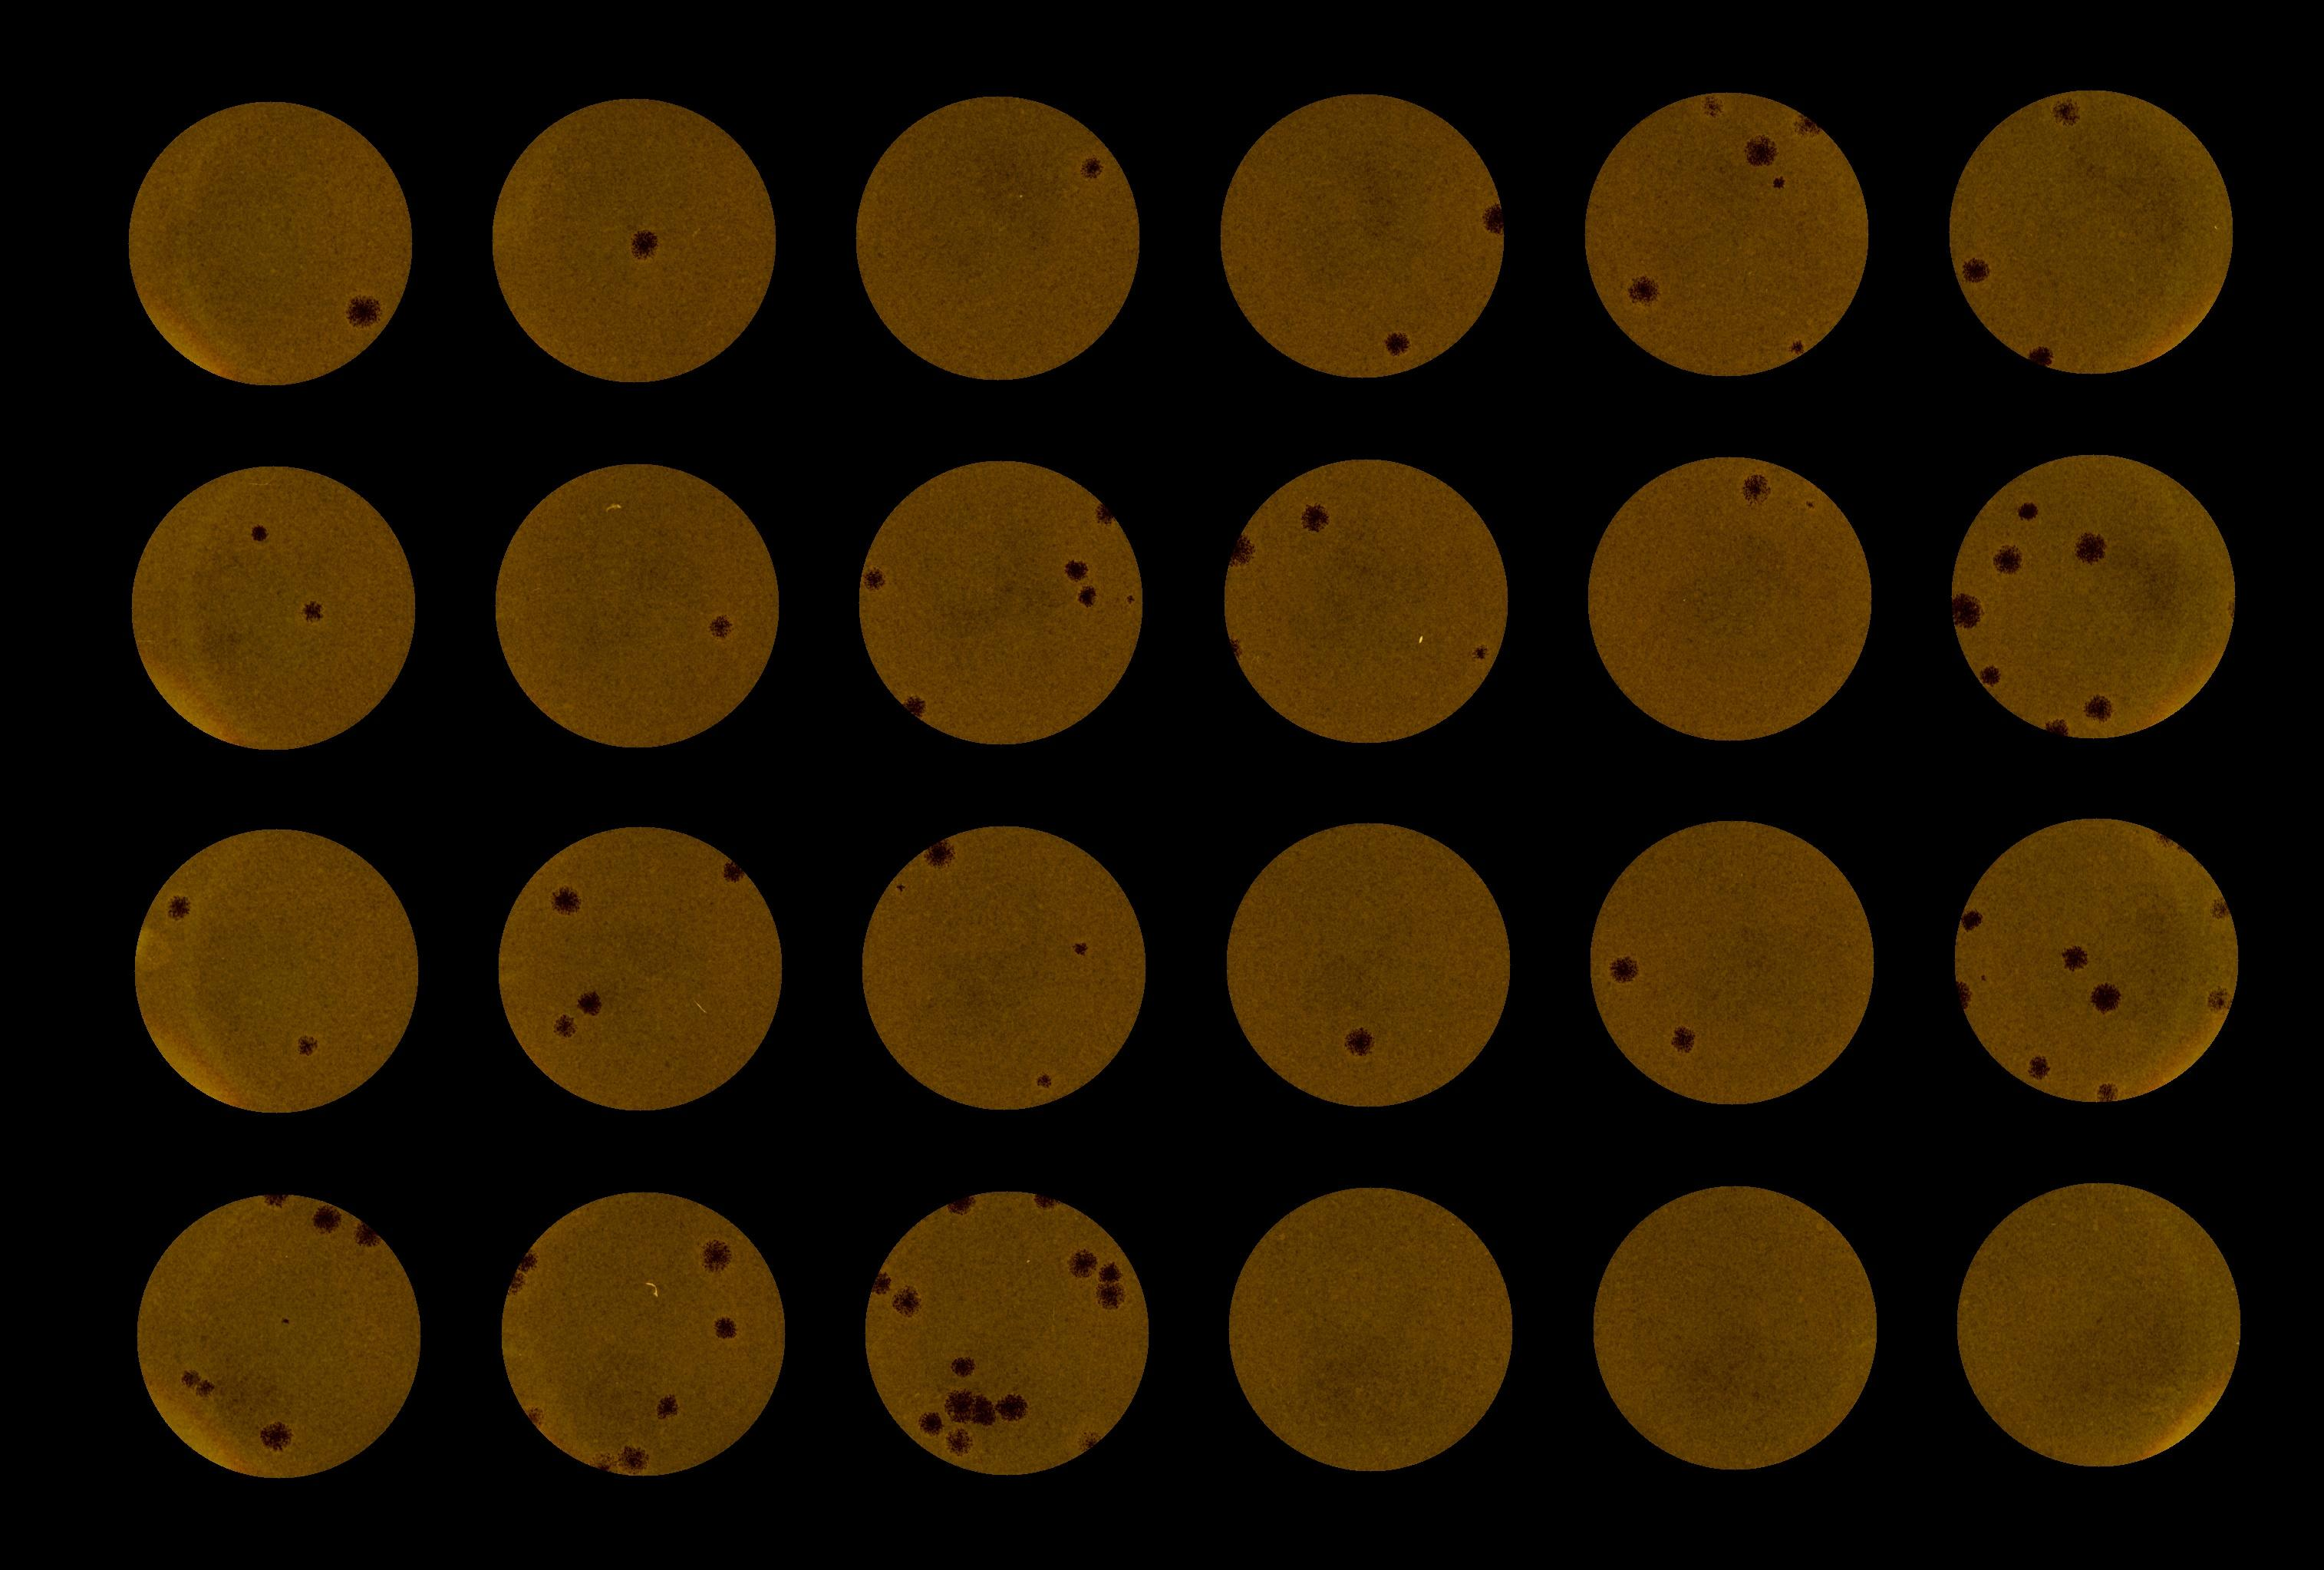
\includegraphics[width=.4\textwidth]{segmentUseRadius.jpg}
\caption{Use of well radius parameter}
\label{fig:segUseRadius}
\end{figure}

\end{enumerate}

Segmentation produces clean regions of interest for each well in the plate. This part of the method is very effective at identifying regions of interest. It exploits the observation that images of plates used for viral plaque studies tend have a similar overall shape. The method expects that the image artifacts that represent the agar or agar equivelant in the wells are the most predominant features of the overall image.    Thus, the image can be reliably eroded until only these features remain.  

Segmentation also exploits the fact that the wells of the tissue plates are machined to be perfectly round[CITE]. This knowledge combined with the well radius parameter that the user provides allows this phase of the method to produce clean regions of interest, which is vastly important to the success of later processing stages.

\subsection{Plaque Structure Counting}
Next remains the task of counting each viral plaque in each well. Given the often noisy nature of the substrate and viral plaques in the well, it’s difficult to devise a method that is accurate for all varieties of input. Viral plaques can be very small, very large, malformed, or even overlapped on top of one other. Nevertheless, the plaque counting method attempts to be simple and accurate for the most commonly occurring instances of viral plaques. It is summarized below.  

\begin{enumerate}
\item Let a masked region of interest be image A. This is a color image containing a single well.
\begin{figure}[H]
\centering
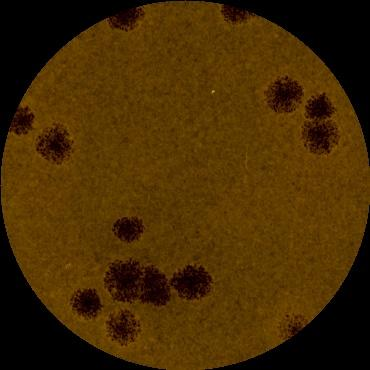
\includegraphics[width=.25\textwidth]{countBegin.jpg}
\caption{Image of a single well, with uninteresting regions masked out}
\label{fig:countBegin}
\end{figure}


\item Grayscale and then apply Otsu thresholding upon image A.
\begin{figure}[H]
\centering
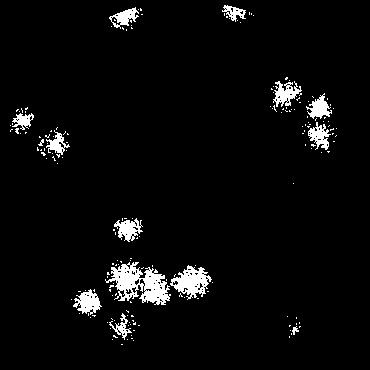
\includegraphics[width=.25\textwidth]{countOtsuA.jpg}
\caption{Otsu thresholding applied to image A}
\label{fig:countOtsuA}
\end{figure}

\item Let images B,C, D, and E be zeroed copies of image A.
\item On image B, render an eroded image.
\begin{enumerate}
\item
Render a morphological open [CITE] operation on image B using a 2x2  rectangular shaped kernel. Choose the number of iterations based on a constant derived from the maximum plaque radius parameter.
\begin{figure}[H]
\centering
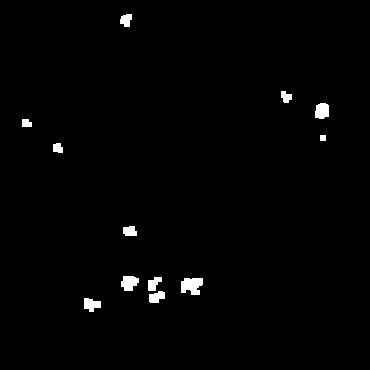
\includegraphics[width=.25\textwidth]{countErodeB.jpg}
\caption{Morphologically eroded rendering of image B.}
\label{fig:countErodeB}
\end{figure}
\end{enumerate}

\item On Image C, render a dilated image.
\begin{enumerate}
\item  Find every contour in A. If the contour area is smaller than a constant derived from the minimum plaque area, remove it from the image.
\item  Dilate C using a 2x2 rectangular shaped kernel. Choose the number of iterations based on a constant derived from the minimum plaque radius parameter.
\item  Perform an  operation similar to the MATLAB imfill() [CITE] on image A to close any internal holes in the contours.
\begin{figure}[H]
\centering
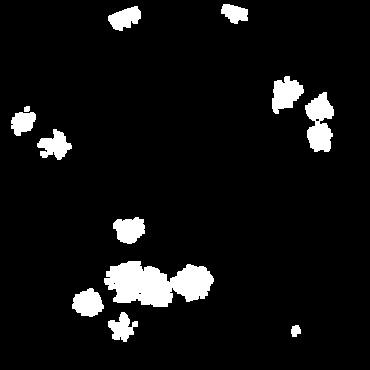
\includegraphics[width=.25\textwidth]{countDilateC.jpg}
\caption{Morphologically dilated rendering of image C.}
\label{fig:countDilateC}
\end{figure}
\end{enumerate}

\item
Merge images B and C into a new image A using a binary image merge of the form 
\begin{verbatim}
A = ~B & C
\end{verbatim}
\begin{figure}[H]
\centering
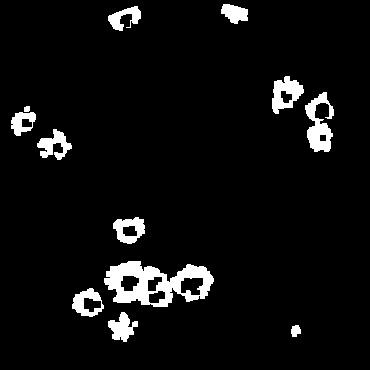
\includegraphics[width=.25\textwidth]{countMerged.jpg}
\caption{Images B and C merged together}
\label{fig:countMerged}
\end{figure}

\item
Obtain the hierarchy of contours in A. Let the total number of contours be determined by the following pseudocode:
\begin{verbatim}

minP = min plaque area
maxP = max plaque area
for contour C in outerContours:
  if( area(C) < minP):
    continue;

  if( area(C) > maxP:
    totalContours += 1;

  totalContours +=
     max(1, innerContourCount) 
\end{verbatim}

\end{enumerate}
The plaque counting method attempts to find a balance between finding feint and sparse plaques VS. properly dividing and detecting dark, prominent plaques. Feint  plaques are typically discovered through analysis of the dilated image (Image C). Dilation effectively joins plaque clusters and forms a cohesive, filled areas. The erosion rendition of the well is focused on discerning prominent plaque structures.  Without an erosion step, a cluster of viral plaque structures are at risk of being inaccurately tallied as a single plaque. Combining the dilated and eroded versions of a well image takes advantages of both morphological transforma ions. Small, feint plaques are emphasized and large  clustered plaques are separated. Both transformations scale with the user supplied parameters maxPlaqueRadius and minPlaqueRadius.

The final step of the per well counting routine considers the max and minPlaqueRadius parameters when tallying total plaque counts. 

\section{Experiments}

For these experiments, a viral plaque images are logically grouped as a study. In a given study, plates are prepared with similar parameters. All of the viral plaque plates in a study have been allowed to incubate for about the same amount of time. Each study consists of plates that use the same or very similar innoculation techniques. The also use similar agar, tissue mediums, and viruses for experiments. This organization scheme allows for a pairing of one set of program parameters to be attached to all the images for a given study. Likewise, parameters are configured for the program on a per study 
basis.

Truth data for each viral plaque well in each plate was obtained by manually counts. These results were compared with data produced by the computer program. Accuracy was measured by finding the sum of errant counts for each well and then dividing that sum by the total truth data count for the well. Errant counts for each well were determined by finding the absolute difference between a count produced by the program and the truth data for a given well.

Each image was aqcuired using an Epson Perfection 799 flat bed scanner, configured to capture at 24 bit color mode and 600 dots per inch. In each experiment, the wells were prepared using a $.5$\%   Methyl Cellulose overlay in lieu of agar. A $.4$\% solution of Crystal Violet was used as a dye as well. 
The plates used in each study were Costar/Corning 24 well (6x4) Tissue culture plates. 

\subsection{Study One}
In the first study, African Green Monkey Kidney Cells  Cell strain Vero E6 were infected with a Vaccinia Virus Western Reserve strain. Seven sample images were captured and sent to the program for processing. Each plate contained 24 wells, and a total of 168 data points were compared with corresponding truth data points.

\begin{figure}[H]
\centering
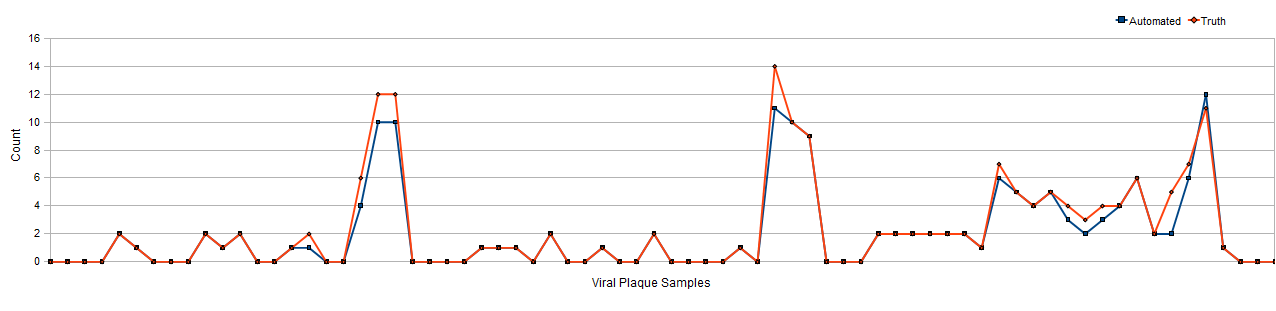
\includegraphics[width=.4\textwidth]{Study1Results.png}
\caption{Study one results}
\label{fig:study1Results}
\end{figure}

\begin{figure}[H]
\centering
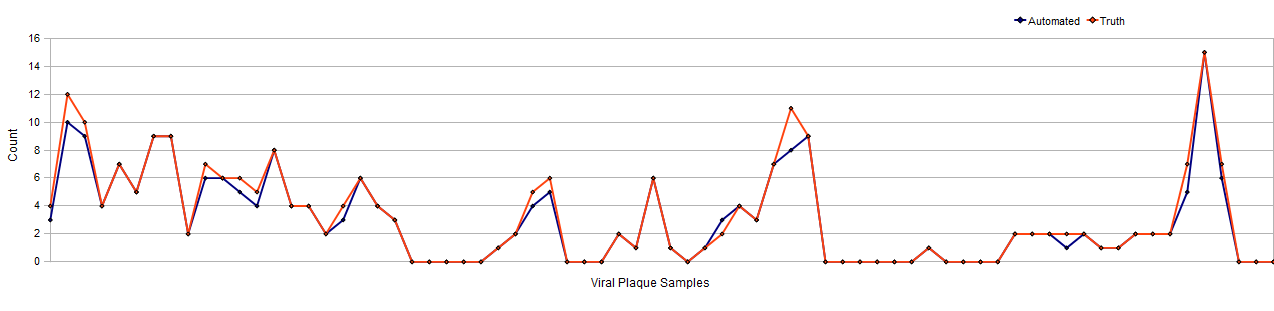
\includegraphics[width=.4\textwidth]{Study1ResultsCont.png}
\caption{Study one results cont.}
\label{fig:study1ResultsCont}
\end{figure}

Total error for study one : $.09$ 


\subsection{Study Two}
In the second study, African Green Monkey Kidney Cells  Cell strain Vero E6 were again infected with Vaccinia Virus Western Reserve strain. Six sample images were captured and sent to the program for processing. Each plate contained 24 wells, and a total of 144 data points were compared with corresponding truth data points.

\begin{figure}[H]
\centering
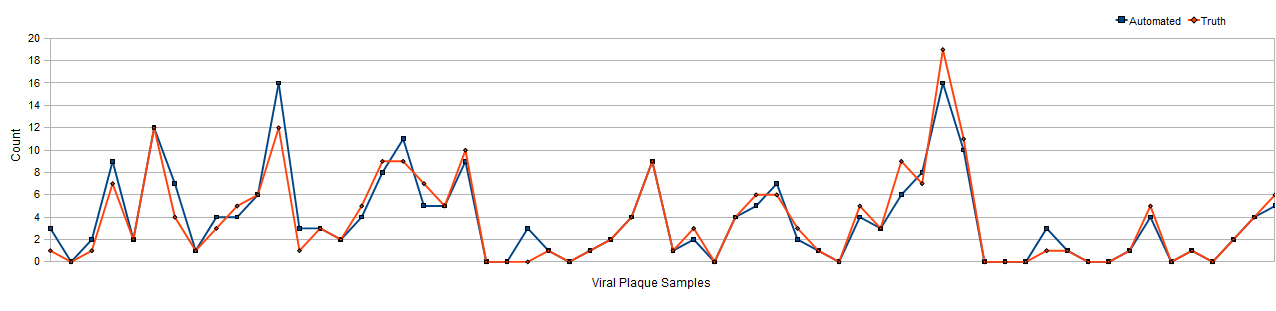
\includegraphics[width=.4\textwidth]{Study2Results.png}
\caption{Study 2 results}
\label{fig:study2Results}
\end{figure}

\begin{figure}[H]
\centering
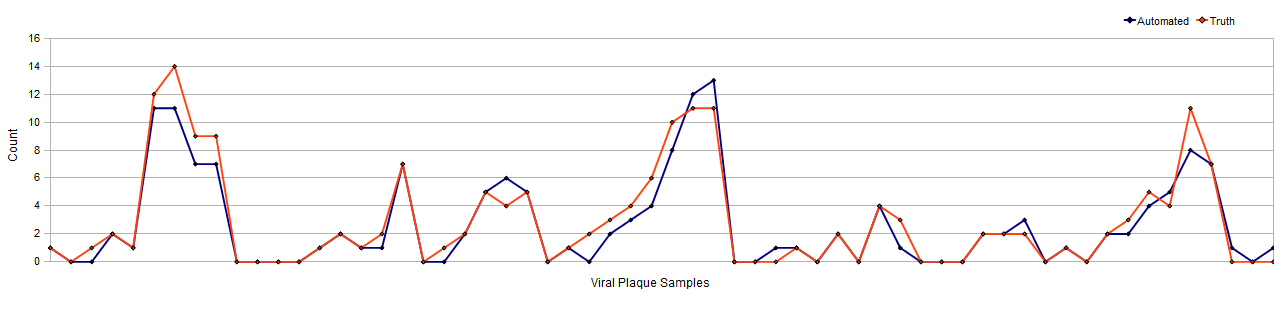
\includegraphics[width=.4\textwidth]{Study2ResultsCont.png}
\caption{Study 2 results cont.}
\label{fig:study2ResultsCont}
\end{figure}
Total error for study two : $.20$ 

\subsection{Study Three}
In the third study, African Green Monkey Kidney Cells  Cell strain Vero E6 were again infected with Monkey Pox Zaire strain. Three sample images were captured and sent to the program for processing. Each plate contained 18 wells, and a total of 52 data points were compared with corresponding truth data points.
\begin{figure}[H]
\centering
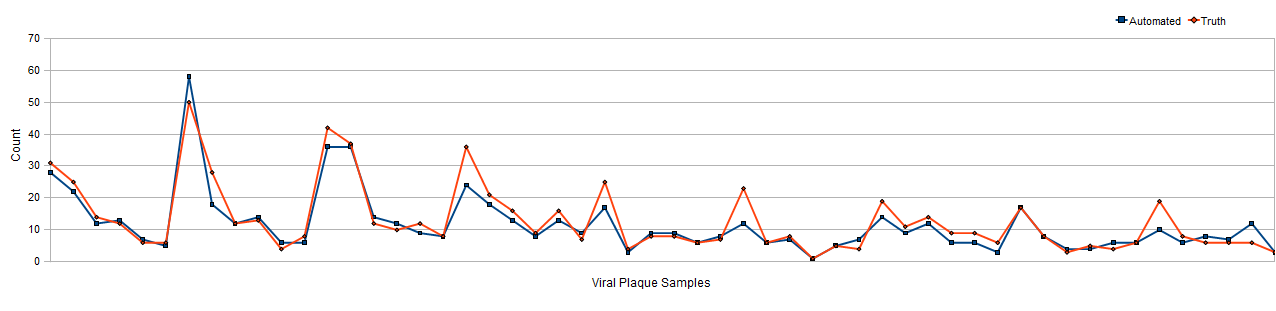
\includegraphics[width=.4\textwidth]{Study3Results.png}
\caption{Study three results}
\label{fig:study3Results}
\end{figure}
Total error for study three: $.20$ 


\section{Discussion}
Experimental data shows that the proposed method is capable of counting entire plates of samples with a recorded accuracy of up to 90 percent.  In some cases, this accuracy is significantly lessened, with a minimum accuracy found to be near 80 percent of truth data in testing. The primary contributors to poor accuracy in these cases is the signal to noise ratio in the images of viral plaque and large discrepencies between the size of plaque structures. Aspects of the innoculation experiments themselves can sometimes produce this noise, though much of it seems to be produced at image acquisition. 

\end{document}

